% ----------------------------------------------------------
% Modelagem do Projeto
% ----------------------------------------------------------
\chapter{Modelagem do Projeto} \label{cha:modelagem}

\section{Levantamento de Requisitos}

\subsection{Requisitos Funcionais}
  Abaixo são listados os requisitos funcionais do sistema: 

  \begin{enumerate}
    \item \textbf{Fornecimento de localização de veículos}: Fornecer informações de localização dos veículos do sistema no momento solicitado.
    \item \textbf{Catálogo de linhas disponíveis no Sistema}: Listar as linhas disponíveis no sistema.
    \item \textbf{Catálogo das paradas de ônibus}: Listar as paradas disponíveis no sistema e as linhas que estão disponíveis em cada uma delas.
    \item \textbf{Avaliação de entidades do sistema}: Registar avaliações dos usuários sobre paradas e veículos do sistema de transporte público.
    \item \textbf{Gerenciamento de usuários e autenticação}: Listar histórico de operações do usuário e ranking de usuários cadastrados.  
  \end{enumerate}

\subsection{Requisitos Não Funcionais}
  Abaixo são listados os requisitos não funcionais do sistema:

  \begin{enumerate}
    \item \textbf{Escalável e de alta disponibilidade}: Deve ser facilmente escalável para atender o aumento repetino de demanda ao mesmo tempo que mantem-se sempre disponível.
    \item \textbf{Baixa carga de trabalho de Infra}: A baixa carga carga baixa de trabalho de infra pode ajudar na evolução da plataforma. 
    \item \textbf{API deve se simples e flexível}: Para ser atrativa ao uso de desenvolvidores a api deve ser bem documentada e flexível.
  \end{enumerate}

\section{Diagramas de casos de uso} \label{sec:modelagem:casos}

O diagrama de caso de uso desenvolvido mostrado na figura \ref{fig:uml_caso_uso} descreve as possíveis interações do usuário através da ferramenta.

\begin{figure}[H]
  \caption{\label{fig:uml_caso_uso}Diagrama UML de Casos de Uso}
  \centering
  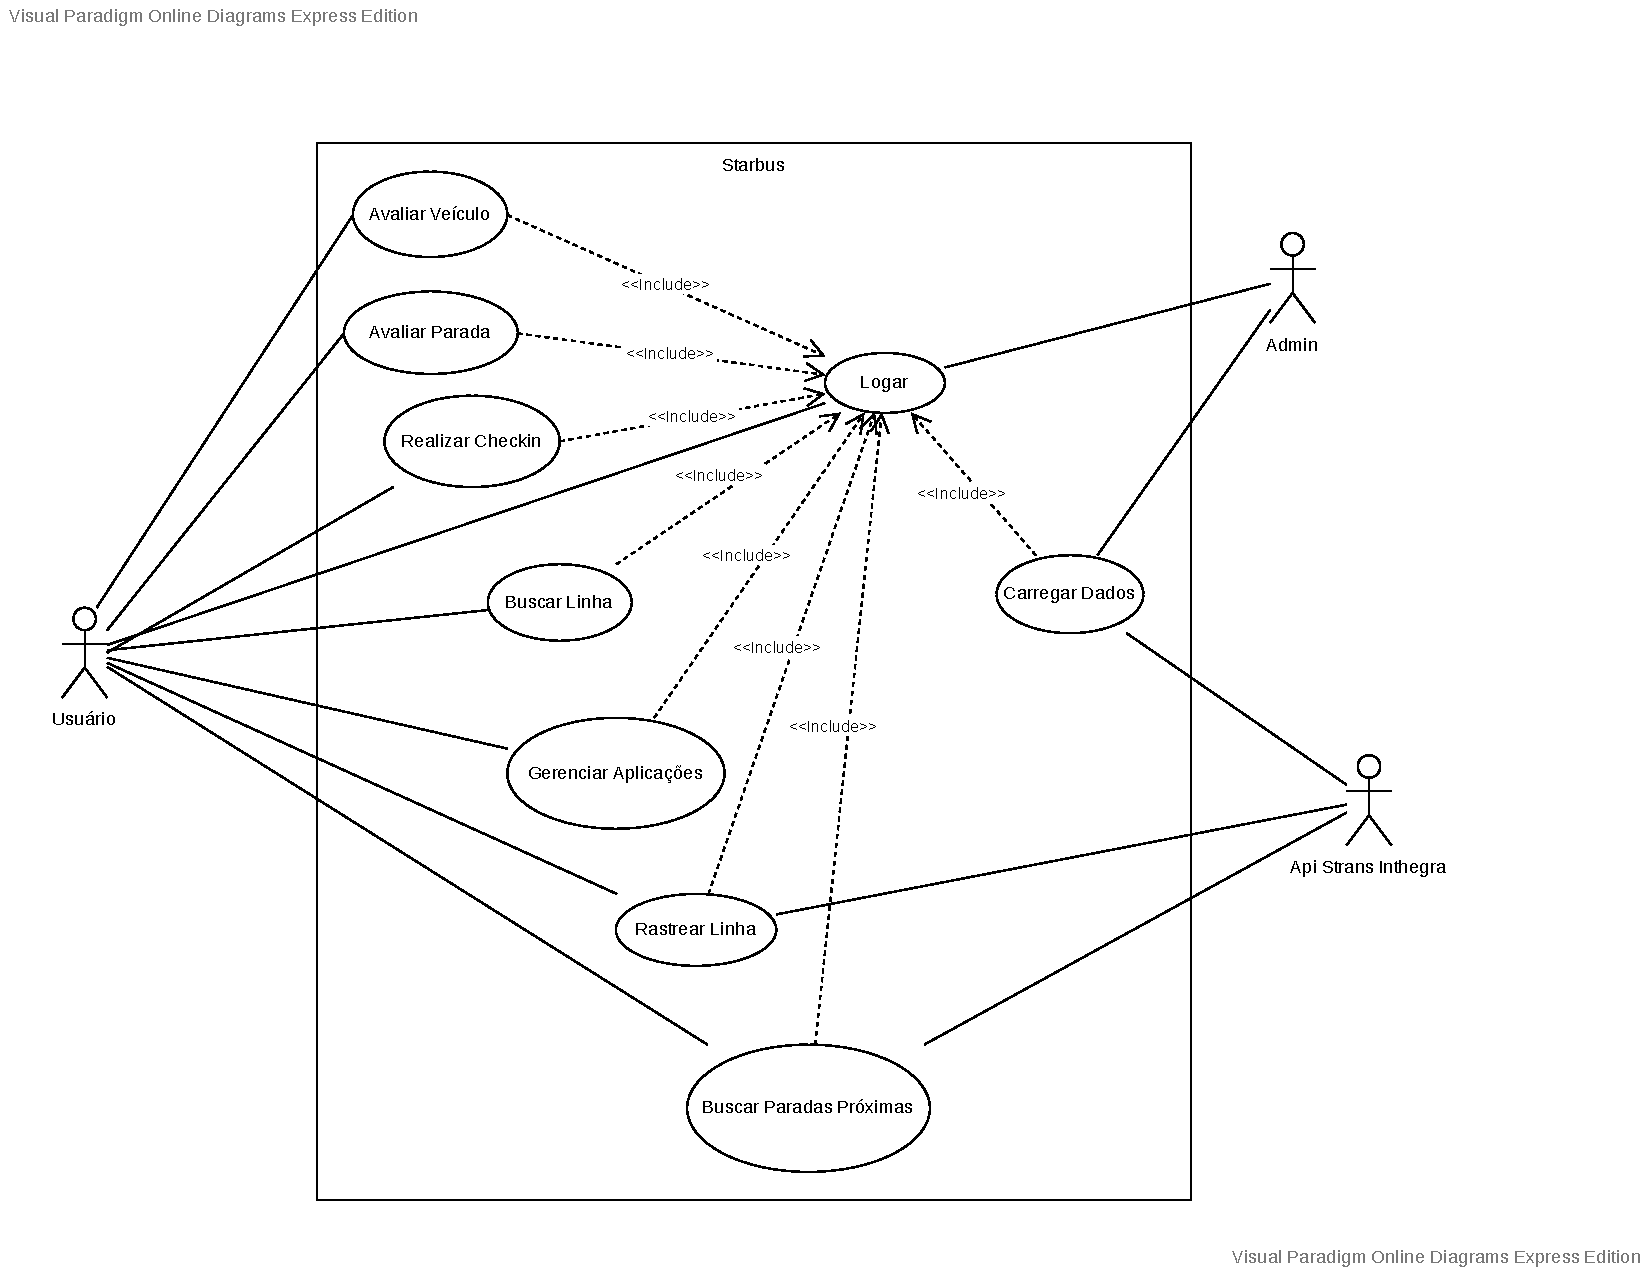
\includegraphics[scale=0.7]{imagens/usecase-sb.pdf}
  \legend{Caso de uso Starbus}
\end{figure}

O diagrama acima expressa os seguintes casos de uso:

\begin{enumerate}
  \item \textbf{Logar}: Ação de identificar-se para fornecer informação para a plataforma, ação necessária para a realização dos casos de uso a seguinte;
  \item \textbf{Carregar Dados}: Usuário pode carregar as informações de linhas e paradas a partir da API Strans Inthegra;
  \item \textbf{Avaliar Veículo}: Usuário devidamente identificado publica sua opinião sobre a parada de ônibus em aspectos como acessibilidade, estado de conservação, lotação e conforto;
  \item \textbf{Avaliar Parada}: Usuário devidamente identificado publica sua opinião sobre a parada de ônibus em aspectos como acessibilidade, estado de conservação, movimentação e conforto;
  \item \textbf{Realizar Checkin}: Usuário devidamente identificado indica que no momento econtra-se em uma devida parada de ônibus ou veículo;
  \item \textbf{Buscar Linha}: Usuário fornece um código ou um termo para pesquisa que é usado para encontrar uma linha que ele deseja detalhes, como itinerário e localização dos veículos;
  \item \textbf{Gerenciar Aplicações}: Um usuário pode ter várias aplicações, aqui ele pode gerencia-las;
  \item \textbf{Rastrear Linha}: Tendo um identificador de uma linha, que pode ser recuperado no caso de uso anterior, consulta a localização dos veículos dessa linha em tempo real com dados fornecidos pela Api Strans Inthegra;
  \item \textbf{Buscar Paradas Próximas}:Usuário fornece uma localização, que pode ser a sua atual ou de um ponto específico que pode quer chegar, a plataforma retorna todas as paradas próximas aquele ponto, com os dados da parada inclusive a avaliação dos usuários sobre a parada;
\end{enumerate}

\section{Diagramas de classe} \label{sec:modelagem:classe}

O modelo de dados da aplicação apresentado na Figura \ref{fig:uml_der}, onde é apresentado um diagrama UML de classes do projeto model.
\begin{lista}
  \item \textbf{User}: Representa um usuário cadastrado do sistema;
  \item \textbf{Asset}: Representa um ativo financeiro;
\end{lista}

\section{Arquitetura do Sistema} \label{sec:modelagem:arquitetura}
\section{Diagrama de Entidades-Relacionamentos} \label{sec:modelagem:der}

Na figura \ref{fig:uml_der} podemos ver a estrutura lógica usada como base para o banco de dados.

\begin{figure}[H]
  \caption{\label{fig:uml_der}Diagrama entidade-relacionamento}
  \centering
  \includegraphics[scale=0.5]{imagens/tfc_der.png}
  \legend{Fonte: Elaborado pelo Autor}
\end{figure}

\section{Interface} \label{sec:modelagem:interface}

\subsection{Tela de Autenticação}
Logo que a aplicação é iniciada é verificado se o usuário já possui sessão ativa, caso não é exibido a tela de autenticação, onde o usuário pode:

\begin{lista}
  \item Acessar utilizando suas credenciais da conta Google;
  \item Acessar como anônimo;
\end{lista}

Em qualquer um dos fluxos escolhidos é criado um registro de usuário, caso não o tenha.

\begin{figure}[H]
  \caption{\label{fig:mock_login}Tela de Autenticação}
  \centering
  \includegraphics[scale=0.4]{imagens/mocks/login.png}
  \legend{Fonte: Elaborado pelo Autor}
\end{figure}

\subsection{Tela Principal}
A primeira tela que um usuário autenticado tem acesso é a tela \textit{home} ou tela principal. Nela são exibidos os seguintes elementos:

\begin{lista}
  \item Um avatar do usuário que leva ao perfil do mesmo;
  \item Saldo atual;
  \item Porcentagem de lucro das últimas 24 horas;
  \item Uma seção que informa a categorial atual da conta;
  \item Um \textit{card} com missões que além de desafiar e guiar o usuário, dão recompensas;
  \item Um \textit{card} para compartilhamento do aplicativo nas redes sociais;
  \item Um \textit{card} para compra do plano sem propagandas;
  \item Um \textit{card} para um módulo de ajuda ao usuário;
  \item \textit{Cards} de acesso aos torneios disponíveis;
\end{lista}

Nessa mesma tela, também podemos ver um menu em \textit{tabs} na parte inferior do aplicativo que auxilia na navegação entre as telas: principal, histórico de \textit{trades} e ranking. E na parte superior que da acesso a tela de perfil do usuário.

\begin{figure}[H]
  \caption{\label{fig:mock_login}Tela Principal}
  \centering
  \includegraphics[scale=0.4]{imagens/mocks/main.png}
  \legend{Fonte: Elaborado pelo Autor}
\end{figure}

\subsection{Tela de Perfil}
Na tela de perfil o usuário tem a possibilidade de restaurar seus dados aos valores iniciais, bem como sair da aplicação e tem acesso alguns indicadores, sendo eles:

\begin{lista}
  \item Portfólio: Valor total;
  \item Dinheiro disponível: Valor total disponível para operação de compra e venda;
  \item Performance: Porcentagem comparativa do saldo atual com o saldo inicial;
  \item \textit{Trades}: Total de negociações realizadas;
  \item Ranking Global: Posição referente a performance realizada e comparada com todos os usuários da plataforma;
  \item \textit{Profitable}: Razão de acertos e total de operações;
\end{lista}

\begin{figure}[H]
  \caption{\label{fig:mock_login}Tela Principal}
  \centering
  \includegraphics[scale=0.4]{imagens/mocks/profile.png}
  \legend{Fonte: Elaborado pelo Autor}
\end{figure}

\subsection{Tela de Histórico}
Na tela de histórico o usuário visualiza todas as negociações já realizadas.

\begin{figure}[H]
  \caption{\label{fig:mock_login}Tela de Histórico}
  \centering
  \includegraphics[scale=0.4]{imagens/mocks/history.png}
  \legend{Fonte: Elaborado pelo Autor}
\end{figure}

\subsection{Tela de Ranking}
A tela de ranking dos usuários é ordenada pelo valor total do portfólio, seguido da porcentagem de lucro da conta, nome, país de origem e avatar.

\begin{figure}[H]
  \caption{\label{fig:mock_login}Tela de Ranking}
  \centering
  \includegraphics[scale=0.4]{imagens/mocks/ranking.png}
  \legend{Fonte: Elaborado pelo Autor}
\end{figure}

\subsection{Tela de Negociações}
Nessa tela, o usuário pode fazer praticamente as mesmas coisas da tela principal, podendo clicar no nome do usuário que publicou a receita e ir para o seu perfil. Com um clique, o usuário também pode curtir, comentar e até mesmo favoritar as receitas. A parte mais importante dessa tela são as informações sobre a receita, onde o usuário pode ver, por exemplo, o tempo de preparo e cozimento, o rendimento e a dificuldade, além de ter todas as informações de ingredientes necessários e modo de preparo para fazer a receita.

Na tela de negociações o usuário acompanha a flutuação do preço dos ativos, cria ordens de compra ou venda, a depender do horário de negociações do mesmo. Na barra superior é exibido saldo, sendo atualizado de acordo com as negociações em andamento. Ainda na barra superior, o usuário pode editar quais ativos de sua preferência devem ser exibidos na listagem horizontal que fica no topo da tela.
No gráfico temos informações referente ao valor do ativo, a valorização do mesmo em relação ao fechamento do dia, o preço médio entre compra e venda, bem como a opção de alterar o tempo do gráfico e dois modos de visualização: em linha ou em barras.

\begin{figure}[H]
  \caption{\label{fig:mock_login}Tela de Negociações}
  \centering
  \includegraphics[scale=0.4]{imagens/mocks/tradezone.png}
  \legend{Fonte: Elaborado pelo Autor}
\end{figure}